\section{Motivation and Scope}

There has been a strong desire for a more space- and/or runtime-efficient
representation for \code{map} among C++ users for some time now.  This has
motivated discussions among the members of SG14 resulting in a
paper\footnote{See P0038R0,
  \href{http://www.open-std.org/jtc1/sc22/wg21/docs/papers/2015/p0038r0.html}{here}.},
numerous articles and talks, and an implementation in Boost,
\code{boost::container::flat_map}\footnote{Part of Boost.Container,
  \href{http://www.boost.org/doc/libs/1_61_0/doc/html/container.html}{here}.}.
Virtually everyone who makes games, embedded, or system software in C++ uses
the Boost implementation or one that they rolled themselves.\\

Here are some numbers that show why.  The graphs that follow show runtimes for
different \code{map}-like associative containers.  The containers used are
Boost.FlatMap, \code{map}, and two thin wrappers over a sorted \code{vector};
the ``custom pair'' version of the sorted \code{vector} uses a simple
\code{struct} instead of \code{pair} for its value type.  All containers use
an \code{int} as the key type and an \code{int} or a \code{struct} with 5
\code{double}s for the value type.\\

All the graphs below were produced on Windows with MSVC 2015.  Similar results
were obtained on Linux, with Clang 3.9 and libc++, and with g++ 4.8.4 and
libstdc++.\\

These four TODO graphs cover the \code{int}-value-type case.  The first graph
shows insertion of N elements with random keys; the second shows full
iteration across all N elements; the third shows \code{map.find()} called once
for each key used in the original insertions; and the fourth shows erasure of
all N elements, by the keys used in the original insertions.

\begin{center}
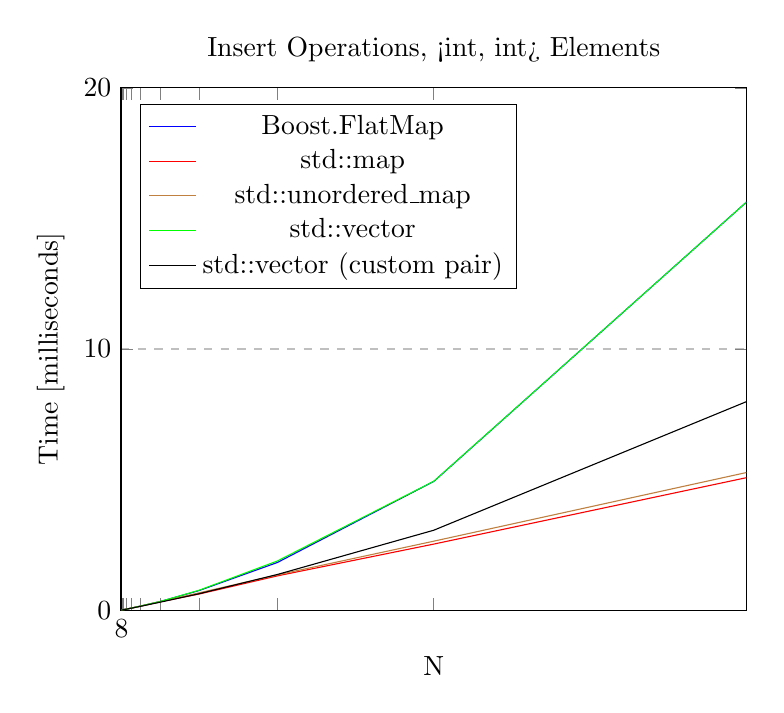
\begin{tikzpicture}[baseline]
    \begin{axis}[
        width=3.75in,
        title={Insert Operations, <int, int> Elements},
        xlabel={N},
        ylabel={Time [milliseconds]},
        xmin=0, xmax=8192,
        ymin=0, ymax=20.0,
        xtick={8,16,32,64,128,256,512,1024,2048,4096,8192,16384},
        xticklabels={8,,,,,,,,,,,},
        ytick={0.0,10.0,20.0,30.0},
        legend pos=north west,
        ymajorgrids=true,
        grid style=dashed,
        scaled x ticks=false,
        scaled y ticks=true,
        legend entries={Boost.FlatMap,std::map,std::unordered\_map,std::vector,std::vector (custom pair)},
        ]

    \addplot[color=blue,mark=|,no markers,]
        coordinates {(8,0.0059498)(16,0.0107412)(32,0.0233666)(64,0.0377144)(128,0.0766718)(256,0.157391)(512,0.33352)(1024,0.754102)(2048,1.8273)(4096,4.93196)(8192,15.629)};

    \addplot[color=red,mark=|,no markers,]
        coordinates {(8,0.0055602)(16,0.0108954)(32,0.0214272)(64,0.0373658)(128,0.0747442)(256,0.153063)(512,0.320434)(1024,0.620922)(2048,1.3154)(4096,2.53239)(8192,5.07565)};

    \addplot[color=brown,mark=|,no markers,]
        coordinates {(8,0.0071926)(16,0.0135076)(32,0.0265528)(64,0.0413182)(128,0.0827056)(256,0.161027)(512,0.33348)(1024,0.665879)(2048,1.35364)(4096,2.64394)(8192,5.27256)};

    \addplot[color=green,mark=|,no markers,]
        coordinates {(8,0.005531)(16,0.0104756)(32,0.0210224)(64,0.0370582)(128,0.076393)(256,0.159561)(512,0.330391)(1024,0.765811)(2048,1.88656)(4096,4.93649)(8192,15.6282)};

    \addplot[color=black,mark=|,no markers,]
        coordinates {(8,0.0056148)(16,0.0106446)(32,0.0199342)(64,0.0366668)(128,0.0742824)(256,0.149897)(512,0.307161)(1024,0.63314)(2048,1.36849)(4096,3.06289)(8192,7.98711)};

    \end{axis}
\end{tikzpicture}
\end{center}
\begin{center}
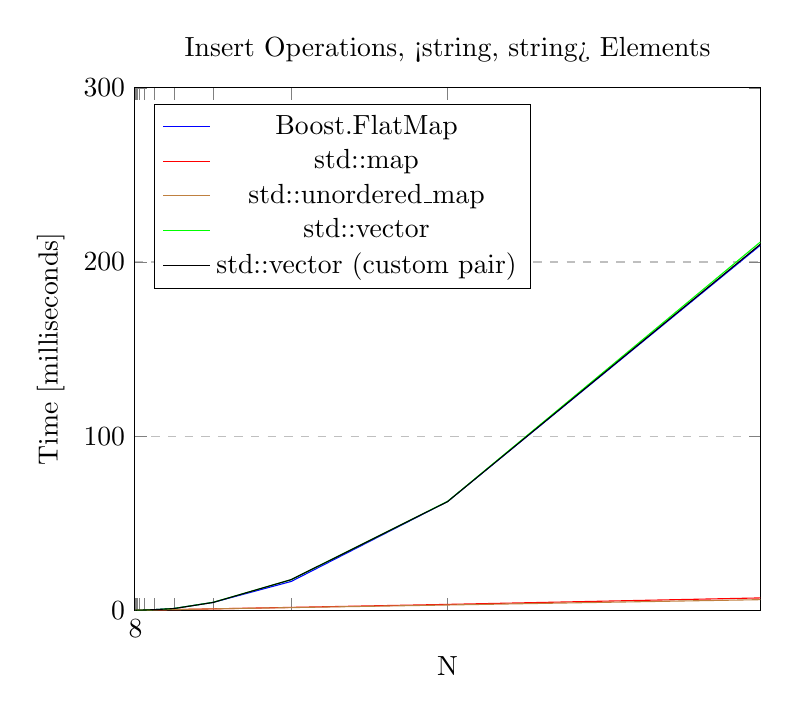
\begin{tikzpicture}[baseline]
    \begin{axis}[
        width=3.75in,
        title={Insert Operations, <string, string> Elements},
        xlabel={N},
        ylabel={Time [milliseconds]},
        xmin=0, xmax=8192,
        ymin=0, ymax=300.0,
        xtick={8,16,32,64,128,256,512,1024,2048,4096,8192,16384},
        xticklabels={8,,,,,,,,,,,},
        ytick={0.0,100.0,200.0,300.0,400.0},
        legend pos=north west,
        ymajorgrids=true,
        grid style=dashed,
        scaled x ticks=false,
        scaled y ticks=true,
        legend entries={Boost.FlatMap,std::map,std::unordered\_map,std::vector,std::vector (custom pair)},
        ]

    \addplot[color=blue,mark=|,no markers,]
        coordinates {(8,0.0057692)(16,0.011579)(32,0.024178)(64,0.053204)(128,0.122083)(256,0.33742)(512,0.990098)(1024,4.47997)(2048,16.5426)(4096,62.4169)(8192,209.624)};

    \addplot[color=red,mark=|,no markers,]
        coordinates {(8,0.00528)(16,0.0105436)(32,0.0211058)(64,0.042245)(128,0.0863456)(256,0.192428)(512,0.375674)(1024,0.790263)(2048,1.62501)(4096,3.35163)(8192,7.06539)};

    \addplot[color=brown,mark=|,no markers,]
        coordinates {(8,0.0058526)(16,0.0116494)(32,0.0234674)(64,0.04889)(128,0.0906308)(256,0.183456)(512,0.369031)(1024,0.780438)(2048,1.50968)(4096,3.0101)(8192,6.06877)};

    \addplot[color=green,mark=|,no markers,]
        coordinates {(8,0.0057404)(16,0.0115094)(32,0.0235232)(64,0.0525768)(128,0.121035)(256,0.33165)(512,1.00852)(1024,4.52587)(2048,17.5152)(4096,62.4831)(8192,211.476)};

    \addplot[color=black,mark=|,no markers,]
        coordinates {(8,0.0054472)(16,0.0112432)(32,0.0231856)(64,0.052171)(128,0.119568)(256,0.32874)(512,0.95423)(1024,4.45803)(2048,17.5896)(4096,62.3912)(8192,210.178)};

    \end{axis}
\end{tikzpicture}
\end{center}

As one might expect, insertionion takes longer in contiguous-storage
implementations.  Boost.FlatMap and a sorted \code{vector<pair<int, int>>}
have superlinear growth in insertion time.  While the curve for sorted
\code{vector} using a custom \code{struct} instead of a \code{pair} is
superlinear as well, it is dramatically flatter in its growth -- much closer
to node-based \code{map}.

\begin{center}
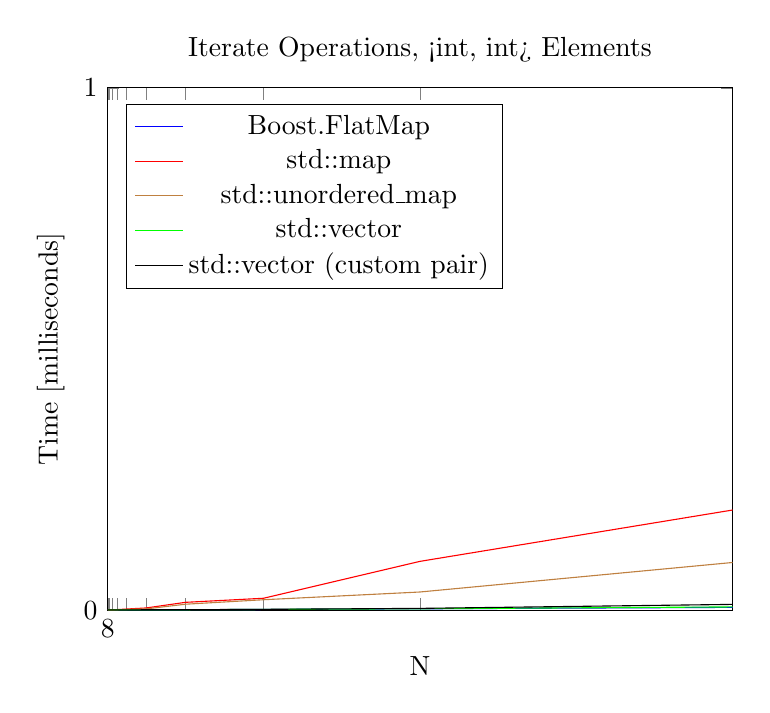
\begin{tikzpicture}[baseline]
    \begin{axis}[
        width=3.75in,
        title={Iterate Operations, <int, int> Elements},
        xlabel={N},
        ylabel={Time [milliseconds]},
        xmin=0, xmax=8192,
        ymin=0, ymax=1.0,
        xtick={8,16,32,64,128,256,512,1024,2048,4096,8192,16384},
        xticklabels={8,,,,,,,,,,,},
        ytick={0.0,1.0,2.0},
        legend pos=north west,
        ymajorgrids=true,
        grid style=dashed,
        scaled x ticks=false,
        scaled y ticks=true,
        legend entries={Boost.FlatMap,std::map,std::unordered\_map,std::vector,std::vector (custom pair)},
        ]

    \addplot[color=blue,mark=|,no markers,]
        coordinates {(8,0.0006288)(16,0.0005868)(32,0.000629)(64,0.0007124)(128,0.0006984)(256,0.0006564)(512,0.000768)(1024,0.000992)(2048,0.001509)(4096,0.0027236)(8192,0.0054754)};

    \addplot[color=red,mark=|,no markers,]
        coordinates {(8,0.0007264)(16,0.0007404)(32,0.0009358)(64,0.0008242)(128,0.001173)(256,0.002305)(512,0.0043582)(1024,0.0150994)(2048,0.022922)(4096,0.0935314)(8192,0.191854)};

    \addplot[color=brown,mark=|,no markers,]
        coordinates {(8,0.0006986)(16,0.0006568)(32,0.0007542)(64,0.000754)(128,0.0009498)(256,0.0014528)(512,0.00257)(1024,0.011496)(2048,0.0200864)(4096,0.0348926)(8192,0.0914082)};

    \addplot[color=green,mark=|,no markers,]
        coordinates {(8,0.0006986)(16,0.0006984)(32,0.000629)(64,0.0005868)(128,0.0006142)(256,0.0006704)(512,0.0007682)(1024,0.0009778)(2048,0.0015502)(4096,0.0028076)(8192,0.0063416)};

    \addplot[color=black,mark=|,no markers,]
        coordinates {(8,0.0006982)(16,0.0007124)(32,0.0005726)(64,0.0005588)(128,0.0006148)(256,0.0007264)(512,0.0008382)(1024,0.0009776)(2048,0.0016766)(4096,0.003534)(8192,0.0111608)};

    \end{axis}
\end{tikzpicture}
\end{center}
\begin{center}
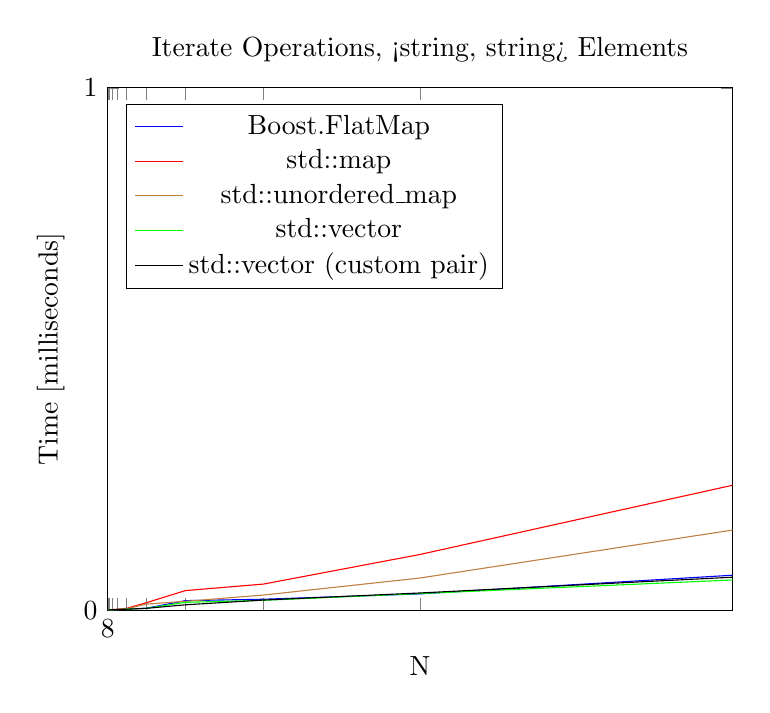
\begin{tikzpicture}[baseline]
    \begin{axis}[
        width=3.75in,
        title={Iterate Operations, <string, string> Elements},
        xlabel={N},
        ylabel={Time [milliseconds]},
        xmin=0, xmax=8192,
        ymin=0, ymax=1.0,
        xtick={8,16,32,64,128,256,512,1024,2048,4096,8192,16384},
        xticklabels={8,,,,,,,,,,,},
        ytick={0.0,1.0,2.0},
        legend pos=north west,
        ymajorgrids=true,
        grid style=dashed,
        scaled x ticks=false,
        scaled y ticks=true,
        legend entries={Boost.FlatMap,std::map,std::unordered\_map,std::vector,std::vector (custom pair)},
        ]

    \addplot[color=blue,mark=|,no markers,]
        coordinates {(8,0.0006006)(16,0.00074)(32,0.00081)(64,0.0009218)(128,0.001271)(256,0.0020536)(512,0.0037436)(1024,0.0183542)(2048,0.0210362)(4096,0.0312606)(8192,0.0670474)};

    \addplot[color=red,mark=|,no markers,]
        coordinates {(8,0.0006282)(16,0.0007406)(32,0.0010054)(64,0.0011872)(128,0.0018436)(256,0.0036458)(512,0.0143314)(1024,0.0376026)(2048,0.0500762)(4096,0.106717)(8192,0.23929)};

    \addplot[color=brown,mark=|,no markers,]
        coordinates {(8,0.0005866)(16,0.0007406)(32,0.0007822)(64,0.0011592)(128,0.0014664)(256,0.0028494)(512,0.0117194)(1024,0.0170136)(2048,0.0290676)(4096,0.06167)(8192,0.153497)};

    \addplot[color=green,mark=|,no markers,]
        coordinates {(8,0.0005866)(16,0.0007262)(32,0.0008802)(64,0.00095)(128,0.001313)(256,0.0020392)(512,0.0035484)(1024,0.015114)(2048,0.0190108)(4096,0.0319314)(8192,0.0578564)};

    \addplot[color=black,mark=|,no markers,]
        coordinates {(8,0.0006982)(16,0.0007404)(32,0.0007682)(64,0.0009638)(128,0.0012992)(256,0.0020112)(512,0.0035756)(1024,0.0103506)(2048,0.0194718)(4096,0.0330208)(8192,0.06322)};

    \end{axis}
\end{tikzpicture}
\end{center}

For all variants but \code{map}, iteration is relatively similar, and much
faster that \code{map}'s.

\begin{center}
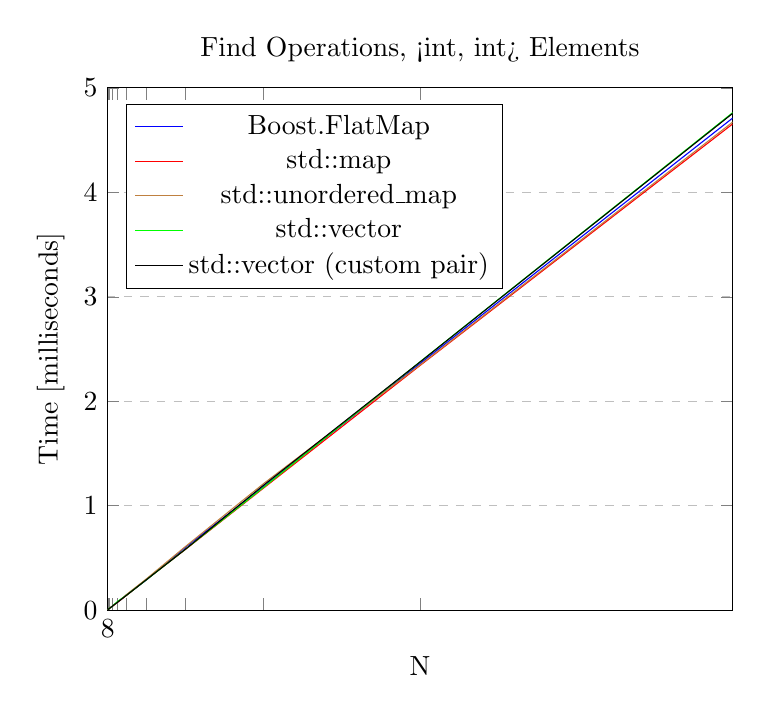
\begin{tikzpicture}[baseline]
    \begin{axis}[
        width=3.75in,
        title={Find Operations, <int, int> Elements},
        xlabel={N},
        ylabel={Time [milliseconds]},
        xmin=0, xmax=8192,
        ymin=0, ymax=5.0,
        xtick={8,16,32,64,128,256,512,1024,2048,4096,8192,16384},
        xticklabels={8,,,,,,,,,,,},
        ytick={0.0,1.0,2.0,3.0,4.0,5.0,6.0},
        legend pos=north west,
        ymajorgrids=true,
        grid style=dashed,
        scaled x ticks=false,
        scaled y ticks=true,
        legend entries={Boost.FlatMap,std::map,std::unordered\_map,std::vector,std::vector (custom pair)},
        ]

    \addplot[color=blue,mark=|,no markers,]
        coordinates {(8,0.0050004)(16,0.0101264)(32,0.0195134)(64,0.035925)(128,0.07202)(256,0.14682)(512,0.289004)(1024,0.60222)(2048,1.18332)(4096,2.35981)(8192,4.71107)};

    \addplot[color=red,mark=|,no markers,]
        coordinates {(8,0.0051402)(16,0.0099592)(32,0.0197228)(64,0.0358706)(128,0.0718094)(256,0.143831)(512,0.292312)(1024,0.581403)(2048,1.169)(4096,2.34158)(8192,4.65476)};

    \addplot[color=brown,mark=|,no markers,]
        coordinates {(8,0.0054198)(16,0.0102104)(32,0.0199606)(64,0.0361356)(128,0.0721862)(256,0.152001)(512,0.29888)(1024,0.609145)(2048,1.21157)(4096,2.34664)(8192,4.67254)};

    \addplot[color=green,mark=|,no markers,]
        coordinates {(8,0.0049588)(16,0.0098902)(32,0.0197514)(64,0.0359402)(128,0.0789338)(256,0.145047)(512,0.290022)(1024,0.583316)(2048,1.17585)(4096,2.37657)(8192,4.76265)};

    \addplot[color=black,mark=|,no markers,]
        coordinates {(8,0.0051118)(16,0.0101694)(32,0.0181044)(64,0.0364722)(128,0.0720058)(256,0.144572)(512,0.291323)(1024,0.583442)(2048,1.19609)(4096,2.37529)(8192,4.75577)};

    \end{axis}
\end{tikzpicture}
\end{center}
\begin{center}
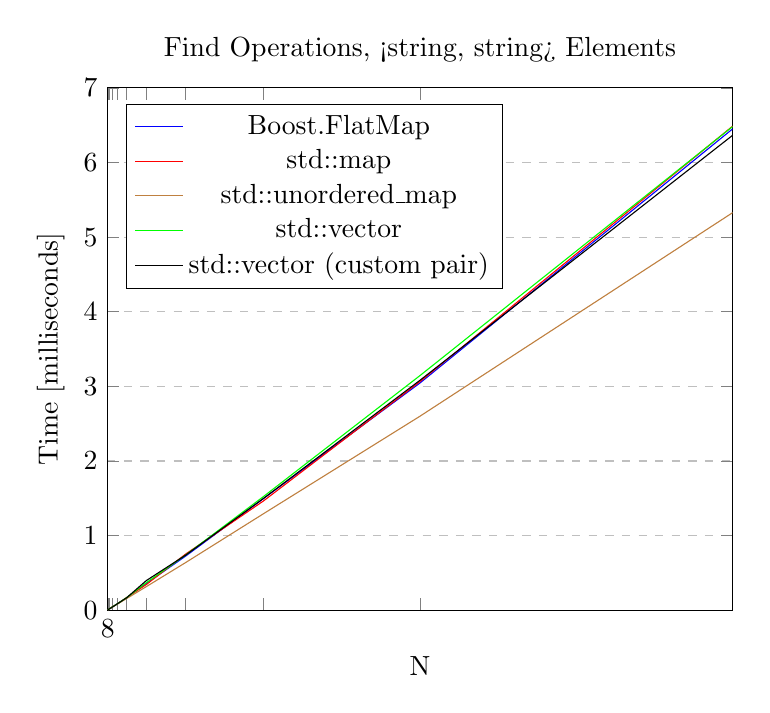
\begin{tikzpicture}[baseline]
    \begin{axis}[
        width=3.75in,
        title={Find Operations, <string, string> Elements},
        xlabel={N},
        ylabel={Time [milliseconds]},
        xmin=0, xmax=8192,
        ymin=0, ymax=7.0,
        xtick={8,16,32,64,128,256,512,1024,2048,4096,8192,16384},
        xticklabels={8,,,,,,,,,,,},
        ytick={0.0,1.0,2.0,3.0,4.0,5.0,6.0,7.0,8.0},
        legend pos=north west,
        ymajorgrids=true,
        grid style=dashed,
        scaled x ticks=false,
        scaled y ticks=true,
        legend entries={Boost.FlatMap,std::map,std::unordered\_map,std::vector,std::vector (custom pair)},
        ]

    \addplot[color=blue,mark=|,no markers,]
        coordinates {(8,0.0048614)(16,0.0098898)(32,0.0198496)(64,0.0399466)(128,0.0814798)(256,0.166729)(512,0.35822)(1024,0.722592)(2048,1.49682)(4096,3.04443)(8192,6.45081)};

    \addplot[color=red,mark=|,no markers,]
        coordinates {(8,0.0047906)(16,0.0098876)(32,0.0194022)(64,0.039278)(128,0.0816864)(256,0.17071)(512,0.343893)(1024,0.749854)(2048,1.46507)(4096,3.06336)(8192,6.48732)};

    \addplot[color=brown,mark=|,no markers,]
        coordinates {(8,0.0050148)(16,0.0098058)(32,0.0196952)(64,0.0462246)(128,0.0778748)(256,0.157142)(512,0.315739)(1024,0.636374)(2048,1.29369)(4096,2.59943)(8192,5.32808)};

    \addplot[color=green,mark=|,no markers,]
        coordinates {(8,0.0049584)(16,0.0101818)(32,0.0202284)(64,0.0408538)(128,0.0829642)(256,0.16993)(512,0.369072)(1024,0.737263)(2048,1.52421)(4096,3.14386)(8192,6.4814)};

    \addplot[color=black,mark=|,no markers,]
        coordinates {(8,0.0049718)(16,0.0102808)(32,0.0198202)(64,0.040497)(128,0.0820482)(256,0.167728)(512,0.396971)(1024,0.735374)(2048,1.49896)(4096,3.08049)(8192,6.36488)};

    \end{axis}
\end{tikzpicture}
\end{center}

\code{find()} performance is roughly similar across all the
implementations, and they all show superlinear growth.  Note that
Boost.FlatMap performs the best here.

\begin{center}
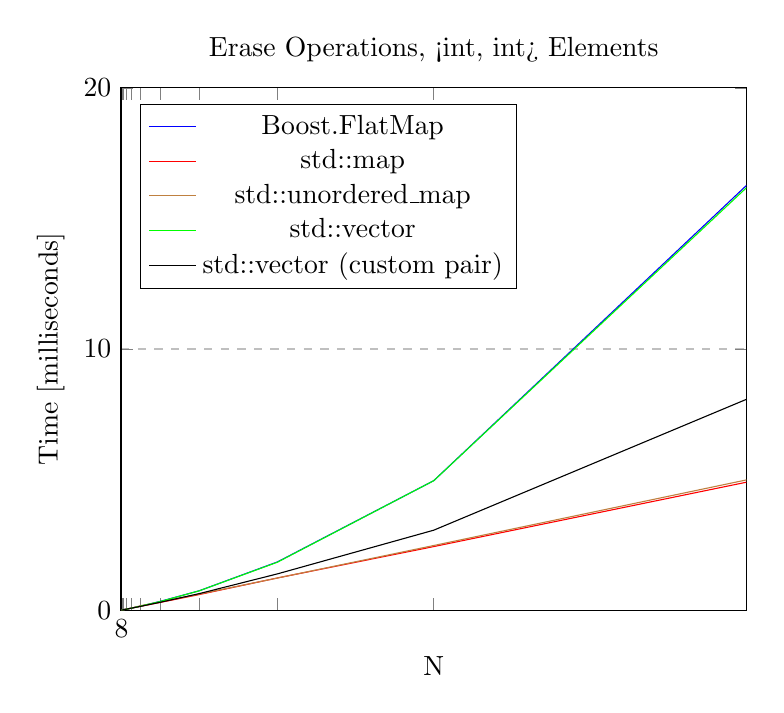
\begin{tikzpicture}[baseline]
    \begin{axis}[
        width=3.75in,
        title={Erase Operations, <int, int> Elements},
        xlabel={N},
        ylabel={Time [milliseconds]},
        xmin=0, xmax=8192,
        ymin=0, ymax=20.0,
        xtick={8,16,32,64,128,256,512,1024,2048,4096,8192,16384},
        xticklabels={8,,,,,,,,,,,},
        ytick={0.0,10.0,20.0,30.0},
        legend pos=north west,
        ymajorgrids=true,
        grid style=dashed,
        scaled x ticks=false,
        scaled y ticks=true,
        legend entries={Boost.FlatMap,std::map,std::unordered\_map,std::vector,std::vector (custom pair)},
        ]

    \addplot[color=blue,mark=|,no markers,]
        coordinates {(8,0.0051126)(16,0.0100848)(32,0.0201984)(64,0.0367362)(128,0.074704)(256,0.155381)(512,0.33682)(1024,0.744706)(2048,1.84875)(4096,4.96076)(8192,16.2665)};

    \addplot[color=red,mark=|,no markers,]
        coordinates {(8,0.0053222)(16,0.0104348)(32,0.0204772)(64,0.036737)(128,0.0735152)(256,0.148946)(512,0.297454)(1024,0.599931)(2048,1.23432)(4096,2.43686)(8192,4.90207)};

    \addplot[color=brown,mark=|,no markers,]
        coordinates {(8,0.0058938)(16,0.0113172)(32,0.0222204)(64,0.0379098)(128,0.075887)(256,0.172089)(512,0.318655)(1024,0.616848)(2048,1.23292)(4096,2.47828)(8192,4.98987)};

    \addplot[color=green,mark=|,no markers,]
        coordinates {(8,0.0052524)(16,0.0102384)(32,0.019793)(64,0.0366096)(128,0.074143)(256,0.154628)(512,0.332809)(1024,0.742556)(2048,1.83816)(4096,4.95925)(8192,16.1788)};

    \addplot[color=black,mark=|,no markers,]
        coordinates {(8,0.0050564)(16,0.0100296)(32,0.0182148)(64,0.036038)(128,0.0746598)(256,0.148581)(512,0.303195)(1024,0.63577)(2048,1.39129)(4096,3.06461)(8192,8.076)};

    \end{axis}
\end{tikzpicture}
\end{center}
\begin{center}
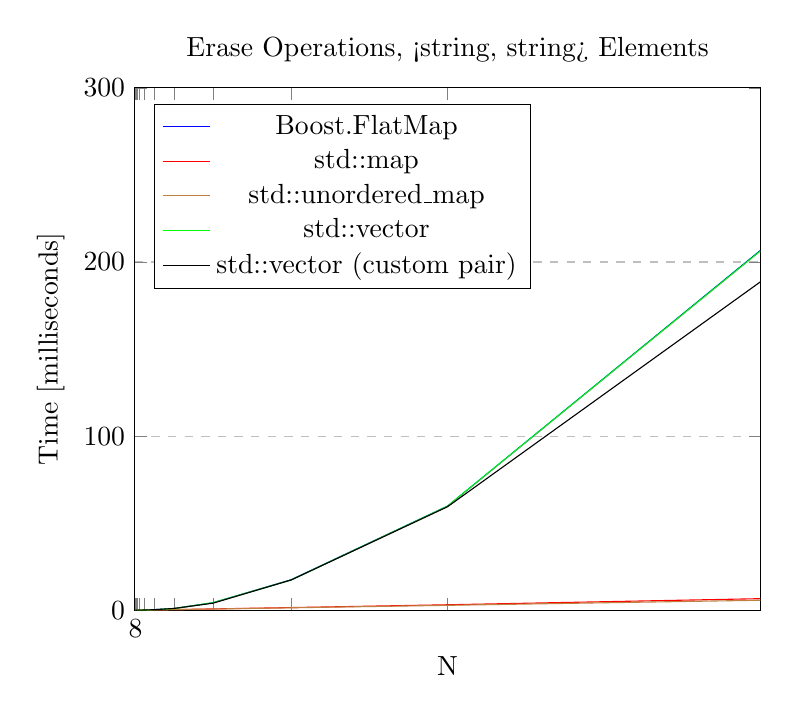
\begin{tikzpicture}[baseline]
    \begin{axis}[
        width=3.75in,
        title={Erase Operations, <string, string> Elements},
        xlabel={N},
        ylabel={Time [milliseconds]},
        xmin=0, xmax=8192,
        ymin=0, ymax=300.0,
        xtick={8,16,32,64,128,256,512,1024,2048,4096,8192,16384},
        xticklabels={8,,,,,,,,,,,},
        ytick={0.0,100.0,200.0,300.0,400.0},
        legend pos=north west,
        ymajorgrids=true,
        grid style=dashed,
        scaled x ticks=false,
        scaled y ticks=true,
        legend entries={Boost.FlatMap,std::map,std::unordered\_map,std::vector,std::vector (custom pair)},
        ]

    \addplot[color=blue,mark=|,no markers,]
        coordinates {(8,0.0051402)(16,0.0105742)(32,0.0231046)(64,0.0501898)(128,0.123534)(256,0.343312)(512,0.978111)(1024,4.29803)(2048,17.5178)(4096,59.8093)(8192,206.596)};

    \addplot[color=red,mark=|,no markers,]
        coordinates {(8,0.0052382)(16,0.0097782)(32,0.0198214)(64,0.039782)(128,0.0819756)(256,0.169683)(512,0.355426)(1024,0.747984)(2048,1.51374)(4096,3.13276)(8192,6.63615)};

    \addplot[color=brown,mark=|,no markers,]
        coordinates {(8,0.0056706)(16,0.0107562)(32,0.0213708)(64,0.0426732)(128,0.0850798)(256,0.170382)(512,0.355751)(1024,0.690397)(2048,1.39315)(4096,2.81999)(8192,5.7266)};

    \addplot[color=green,mark=|,no markers,]
        coordinates {(8,0.0054194)(16,0.0107006)(32,0.0232002)(64,0.0498932)(128,0.122992)(256,0.309713)(512,0.958439)(1024,4.33429)(2048,17.3789)(4096,59.7579)(8192,206.238)};

    \addplot[color=black,mark=|,no markers,]
        coordinates {(8,0.005267)(16,0.0106154)(32,0.0227708)(64,0.0493912)(128,0.122177)(256,0.310864)(512,1.01431)(1024,4.05284)(2048,17.3823)(4096,59.4496)(8192,188.58)};

    \end{axis}
\end{tikzpicture}
\end{center}

Erasure has a similar performance profile to insertion, except that the sorted
\code{vector<pair<int, int>>} performs substantially better than
Boost.FlatMap.\\


\subsection{Implications}

TODO Iteration is vastly cheaper for contiguous-storage variants.  It has been
suggested that a \code{map} with a custom allocator can achieve similar
performance to flat data structures, but this would not apply to iteration
performance, unless the values were added to the \code{map} in sorted order.\\

In all the graphs above, the reason the custom-\code{pair} sorted vector
performs so much better than \code{vector<pair<int, int>>} seems to be that
the custom-\code{pair} type has \code{nothrow} special functions.
Implementing all the special functions and adding \code{nothrow(false)} to
each makes the custom-\code{pair} version perform identically to the
\code{pair<int, int>} version.

Boost.FlatMap differs quite a bit from a sorted \code{vector}.  Clearly there
are a lot of QOI choices to make in implementing a standard \code{flat_map}.
